\chapter{Zusammenfassung und Ausblick}
\label{chap.zusammenfassung}
%\red[TODO:\\
%Entwickeltes System kurz zusammenfassen, beginnend damit warum es erstellt wurde!\\
%Ergebnisse und Fazit daraus kurz zusammenfassen\\
%Ausblick geben auf erweiterungen des Systems - Um die Einsschränkungen zu beheben - Um das System zu erweitern/verbessern\\
%Ausblick geben auf mögliche Anwendungsfälle/-gebiete\\
%Limitierungen in Ausblick aufnehmen\\
%]

%\red[Allgemein, was wurde aufgebaut, warum, welche Komponenten!?\\]%
In dieser Arbeit wurde der Aufbau eines handführbaren \kps{} beschrieben, welches die interaktive Darstellung visueller Zusatzinformationen in bekannten Umgebungen ermöglicht. Anhand eines realistischen Anwendungsfalls konnte der Funktionsumfang des entwickelten Systems dargestellt werden.\\

Existierende handführbare Projektionssysteme werden in verschiedenen Bereichen im Rahmen von \textit{Augmented-Reality}-Anwendungen eingesetzt. Die Lokalisation der Systeme innerhalb der Umgebungen basiert dabei meist auf externen Messeinrichtungen. Die Selbstlokalisation mobiler Systeme stellt gleichzeitig jedoch insbesondere in der Robotik einen aktuellen Forschungsansatz dar. Das aufgebaute \kps{} kombiniert diese beiden Forschungsbereiche und stellt damit ein flexibles System zur interaktiven Visualisierung virtueller Daten dar.\\

Als technologische Grundlage des Systems wurden eine RGB-D Kamera und ein Pico-Laser-Projektor in einem gemeinsamen Aufbau kombiniert. Zunächst wurde eine Kalibrierung der RGB-D Kamera durchgeführt, um eine präzise Vermessung der Umgebung zu ermöglichen. Darauf aufbauend wurde der Projektor kalibriert und seine relative Lage bezüglich des Kamerasystems bestimmt, wodurch die Transformations- und Abbildungsvorschriften des \kps{s} bezogen auf die Umgebung festgelegt werden konnten.\\

Ein modularer Softwareaufbau bildet die verschiedenen Funktionsbereiche des Systems ab. Um den Datenaustausch zwischen den Komponenten zu ermöglichen, wurden diese an das Meta-Betriebssystem ROS angebunden. Der Anwendungsumfang kann damit durch Austausch oder Modifikation einzelner Module bei Bedarf erweitert werden.\\

Die Basis der Anwendung bildet eine Datengrundlage, welche die reale Umgebung abbildet und die Ergänzung virtueller Objekte ermöglicht. Basierend auf dieser virtuellen Umgebung wurde die Selbstlokalisation des Systems realisiert. Das eingesetzte globale Lokalisationsverfahren des \textit{Monte-Carlo-Algorithmus} ermittelt über ein Partikelfilter eine initiale Approximation der Systempose innerhalb der Umgebung. Dazu werden die Sensordaten der Tiefenkamera ausgewertet und mit der Modellumgebung abgeglichen. Durch Bestimmung visueller Odometriedaten wird anschließend die Bewegung des Systems verfolgt. Um zusätzliche Lagedaten für die Lokalisation zu ermitteln, wurde eine inertiale Messeinheit in das System integriert.\\

Durch die Anbindung des Projektors können dem Benutzer virtuelle Daten lagerichtig in der realen Umgebung visualisiert werden. Die Bilddaten dafür werden durch Simulation der Projektorperspektive innerhalb der Modellumgebung generiert. Um die perspektivische Abbildung zu bestimmen, werden dabei die Parameter des realen Projektors verwendet, welche im Rahmen der Kalibrierung bestimmt wurden.\\

Die Interaktion des Benutzers mit der projizierten Darstellung vervollständigt den Anwendungsumfang des aufgebauten \kps{s}. Es wurde dazu ein Ansatz implementiert, welcher dem Benutzer die Auswahl und Modifikation der virtuellen Objekte durch Zeigebewegungen ermöglicht. Die direkte Kopplung mit der Visualisierung ermöglicht eine interaktive Projektion bei gleichzeitiger Aktualisierung der Datengrundlage, wodurch eine Rückführung in den virtuellen Planungsprozess entsteht.\\

Abschließend wurde eine experimentelle Auswertung der Lokalisation und Visualisierung durchgeführt. Während für die Projektionsgenauigkeit innerhalb der Visualisierungsebene nur geringe Abweichungen gemessen wurden, zeigte sich, dass die aus den Verfahren zur globalen und lokalen Lokalisation ermittelte Pose mit deutlichen Ungenauigkeiten behaftet ist. Die Eignung des \kps{s} im Rahmen hoch genauer Visualisierungen wird dadurch bei aktueller Konfiguration eingeschränkt.\\
%Die Fehlereinflüsse sind dabei jedoch nicht auf das Funktionsprinzip selbst, sondern hauptsächlich auf Limitierungen der Rechenkapazität zurückzuführen.\\

Im Folgenden soll ein Ausblick auf Möglichkeiten zur Steigerung der Lokalisationsgüte gegeben werden. Zusätzlich werden Modifikationen und Ergänzungen diskutiert, welche Optionen zur Weiterentwicklung des \kps{s} darstellen.\\

Die Genauigkeit der globalen Lokalisation ist direkt abhängig von der gewählten Anzahl an Partikeln. Eine Verringerung der zu betrachtenden Freiheitsgrade im Partikelfilter führt demnach bei konstanter Partikelanzahl dazu, dass die verbleibenden Freiheitsgrade mit höherer Auflösung bestimmt werden können. Diese Reduzierung der freien Parameter könnte beispielsweise durch Einsatz eines elektronischen Kompass zur Bestimmung des Gier-Winkels erreicht werden. Derartige Systeme sind zwar besonders in Innenräumen verschiedenen Störeinflüssen ausgesetzt, durch geeignete Kalibrierverfahren können jedoch Genauigkeiten im Bereich weniger Grad erzielt werden \cite{Li2011}. Da die Anzahl betrachteter Partikel bereits bei Approximation des Gier-Winkels deutlich reduziert werden könnte, sollte diese Möglichkeit in weiteren Untersuchungen näher evaluiert werden. Auch die Robustheit der lokalen Lokalisation könnte damit gesteigert werden, indem das EKF neben den Orientierungsdaten der IMU auch den Gier-Winkel in die Sensorfusion integriert. Eine geeignete Schnittstelle zur Anbindung weiterer Sensoren liegt dabei in Form des verwendeten Arduino bereits vor.\\

Eine weitere Möglichkeit die Genauigkeit der globalen Lokalisation zu erhöhen liegt in der Berücksichtigung einer variablen Varianz des Sensormodells. Wie \textsc{Khoshelham} und \textsc{Elberink} \cite{Khoshelham2012} zeigen konnten, weist diese für die Kinect eine nichtlineare Abhängigkeit von der Messdistanz auf. Insbesondere für das RCM könnte dies zu einer deutlichen Steigerung der Lokalisationsgüte führen.\\

Durch die Implementierung zusätzlicher Lokalisationsverfahren könnte die Systempose ebenfalls mit höherer Genauigkeit ermittelt werden. Das in \kapitel{chap.unimod} beschriebene \textit{Scan Matching} könnte bei erfolgreicher Approximation der Systempose eine Optimierung der Überdeckung zwischen Modell- und Sensordaten bestimmen. Als Basis dafür wäre die Bestimmung einer Metrik erforderlich, welche eine zuverlässige Aussage darüber ermöglicht, ob die Pose korrekt angenähert wurde oder eine fehlerhafte globale Lokalisation vorliegt.\\

Abschließend wäre bei Erhöhung der zur Verfügung stehenden Rechenkapazität eine generelle Steigerung der Lokalisationsgenauigkeit zu erwarten. In der globalen Lokalisation könnte sowohl die Partikelanzahl als auch die Auflösung der betrachteten Punktwolke erhöht werden. Die Berechnung der visuellen Odometrie könnte voraussichtlich mit höherer Frequenz durchgeführt werden, wodurch eine präzisere Bestimmung der veränderten Pose möglich wäre.\\

Die Auswertung der Projektionsgenauigkeit ergab innerhalb der Visualisierungsebene nur geringe Fehlerwerte. Eine Integration der durch die externe Kamera ermittelten Messdaten in den Kalibrierungsvorgang könnte jedoch genutzt werden, um die Projektionsgenauigkeit zu erhöhen und die Fehlerwerte bezüglich der Tiefendarstellung zu verringern. Über einen iterativen Prozess wäre so die Korrektur der während der Kalibrierung ermittelten Parameter möglich.\\

Bezüglich der Visualisierung wäre ein höherer Kontrast der Projektion auch bei weiteren Entfernungen zur Projektionsfläche anzustreben. Der eingesetzte Laser-Projektor verfügt über eine Helligkeit von 15 Lumen, weshalb es bei einem Projektionsabstand über \SI{2}{\meter} zu deutlichen Kontrastverlusten kommt. Ein höherer Helligkeitswert könnte kontrastreichere Abbildungen erzeugen. Die Leistung und damit auch die Helligkeit ist bei Laser-Projektoren jedoch durch die zulässige Laser-Klasse vorgegeben. Besonders im Bereich der tragbaren Projektoren sollte die Laser-Klasse 2\footnote{Klassifizierung nach EN 60825-1} nicht überschritten werden, da es sonst bei versehentlicher Betrachtung des Laserstrahls zu permanenten Schädigungen der Netzhaut kommen kann.\\

Um dennoch höhere Kontrastverhältnisse zu erzielen, könnte die Umgebungsausleuchtung verringert werden. Da die visuelle Odometrie allerdings eine ausreichende Ausleuchtung der Umgebung erfordert, um die Merkmale im RGB-Bild robust bestimmen zu können, kann die Beleuchtungsstärke der Umgebung nur bis zu einem gewissen Grenzbereich abgesenkt werden. Als Lösung zur Erhöhung des Kontrastes verbleibt daher der Einsatz von Softwarekonzepten. \textsc{Bimber} \textit{et al.} \cite{Bimber2005} stellen eine Methode vor, welche die Projektion bezüglich Farb- und Geometriedarstellung an beliebige Untergründe anpasst. Zur Ermittlung der Umgebungsinformationen wird dabei eine Kamera eingesetzt. Eine Anwendung dieses Prinzips im Rahmen des aufgebauten \kps{s} wäre somit ohne Modifikationen der verwendeten technologischen Komponenten möglich.\\ 

Durch den minimalen aufgelösten Tiefenwert des Microsoft Kinect Sensors von \SI{0,5}{\meter} ergibt sich eine Limitierung der aktuellen Systemkonfiguration bezüglich der Benutzerinteraktion. Um die Zeigerichtung robust erkennen zu können, ist es erforderlich, dass der Nutzer die Auswahl und Modifikation der Modellobjekte mit ausgestrecktem Arm durchführt. Eine kürzere minimale Distanz würde den Komfort bei der Eingabe deutlich erhöhen, da so die Interaktion bei verschiedenen Haltungen möglich wäre und der Benutzer bei längerer Interaktionsdauer entlastet würde. Dies könnte beispielsweise durch Erweiterung der Systemkomponenten um eine zusätzliche IR-Kamera für den Nahbereich erreicht werden, wie in der von \textsc{Molyneaux} \textit{et al.} \cite{Molyneaux2012} vorgestellten Arbeit. Eine Evaluierung des implementierten Interaktionsansatzes im Rahmen von Benutzerstudien sollte darüber hinaus durchgeführt werden, um weiteres Optimierungspotenzial bezüglich Komfort und Präzision der Benutzereingabe zu ermitteln.\\

Die Vielseitigkeit des aufgebauten Systems führt zu Einsatzmöglichkeiten, die über den Kontext des in dieser Arbeit beschriebenen Anwendungsfalls hinausgehen. Die Unabhängigkeit der Lokalisation von externen Messeinrichtungen erhöht die Flexibilität gegenüber existierenden handführbaren Projektionssystemen dabei deutlich. Durch zukünftige technologische Fortschritte werden die Limitierungen der aktuellen Systemkonfiguration in den Hintergrund treten. Das aufgebaute \kps{} stellt in Zusammenhang mit dem erstellten Softwarekonzept eine funktionsfähige Lösung dar, virtuelle Modelldaten in der Realität zu visualisieren und zu modifizieren.


%\section{Interaktion}
%Durch den minimalen aufgelösten Tiefenwert des Microsoft Kinect Sensors von \red[ABSTAND 0,5m?] ergibt sich eine Limitierung der aktuellen Systemkonfiguration bezüglich der Benutzerinteraktion. Um die Zeigerichtung robust erkennen zu können, ist es erforderlich, dass der Nutzer die Auswahl und Modifikation der Modellobjekte mit ausgestrecktem Arm durchführt. Eine kürzere minimale Distanz würde den Komfort bei der Eingabe deutlich erhöhen, da so die Interaktion bei verschiedenen Haltungen möglich wäre und der Benutzer bei längerer Interaktionsdauer entlastet werden würde.\\
%
%Der minimale Tiefenwert definiert darüber hinaus auch den minimalen Abstand zur Projektionsfläche, da sowohl der globalen als auch der lokalen Lokalisation bei Unterschreiten dieses Abstands keine Umgebungsinformationen mehr zur Verfügung stehen. Es ergibt sich daraus zusammen mit dem definierten maximalen Projektionsabstand der in \abb{fig.optdist} dargestellte optimale Anwendungsabstand.\\
%\red[Interaktionsbereich hier auch einzeichnen! Wand anstelle rotem Endbereich!?\\]
%
%\begin{figure}[!ht]
%	\begin{center}
%		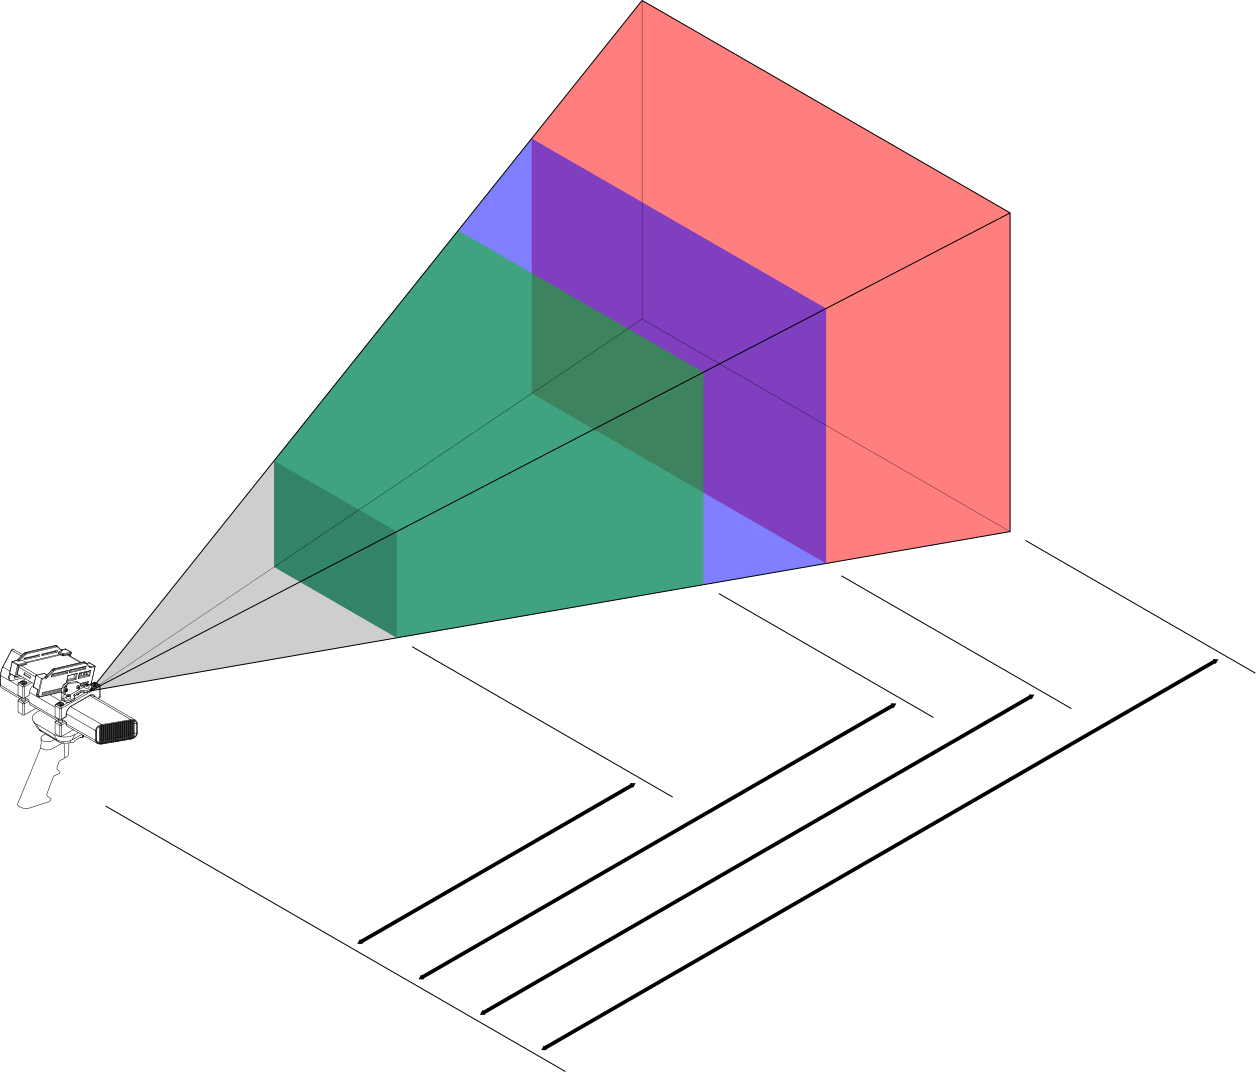
\includegraphics[scale=0.25]{anwendungsbereich}
%		\caption{Optimaler Abstand während der Verwendung des \kps{s}}
%		\label{fig.optdist}
%	\end{center}
%	%\vspace*{-8mm}
%\end{figure}


% Dadurch kommt es bei Projektionen in stark ausgeleuchteten Umgebungen und bei größeren Entfernungen zur Projektionsfläche zu einem deutlichen Kontrastverlust. Ein höherer Helligkeitswert würde somit den Anwendungsbereich erweitern. Diese Anforderung steht damit jedoch im Kontrast zu der Anforderung ausreichender Umgebungsausleuchtung für eine robuste visuelle Odometrie. Die Auswirkungen unterschiedlicher Beleuchtungsstärken der Umgebung zeigt \abb{fig.optlight}. Im Anwendungsfall gilt es somit, einen Kompromiss zu finden, welcher beiden Anforderungen gerecht wird.\\
%\red[In Kontrast setzen zu Anforderungen des Projektors -> optimale Helligkeit in der Mitte; Bilder für alle drei Anwendungsfälle aufnehmen?\\]

%\begin{figure}[!ht]
%	\begin{center}
%		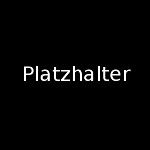
\includegraphics[scale=1.0]{spacer}
%		\caption{Optimaler Helligkeitsbereich/Bilder die verdeutlichen wann visodom failt und wann Projektion zu undeutlich wird}
%		\label{fig.optlight}
%	\end{center}
%	%\vspace*{-8mm}
%\end{figure}

%Anzumerken bleibt, dass eine Begrenzung der Leistung und damit auch der Helligkeit bei Laser-Projektoren durch die zulässige Laser-Klasse vorgegeben ist. Besonders im Bereich der tragbaren Projektoren sollte die Laser-Klasse 2\footnote{Klassifizierung nach EN 60825-1} nicht überschritten werden, da es sonst bei versehentlicher Betrachtung des Laserstrahls zu permanenten Schädigungen der Netzhaut kommen kann. Auch im Hinblick auf die \red[zuvor besprochene] Umgebungsausleuchtung sollte bei der Anwendung deshalb ein maximaler Abstand von etwa \red[TODO] zur Projektionsfläche nicht überschritten werden.\\

%Eine weitere Möglichkeit eine deutlichere Darstellung der visuellen Zusatzinformationen zu erreichen, wäre neben einer Kontrast- beziehungsweise Helligkeitserhöhung auch eine Erhöhung der Auflösung der Projektion. Der ShowWX ist auf eine Auflösung von 480p begrenzt, wodurch es besonders bei feineren Strukturen trotz der Laser-Technologie zu unscharfen Abbildungen kommen kann.\\





%\red[globale Lokalisation erfordert eindeutige features in der Karte -> schon während der Lokalisation nennen?\\]

%Die vorgestellten Verfahren zur Selbstlokalisation und Darstellung visueller Zusatzinformationen für den Anwender sind allgemein anwendbar und hardwareunabhängig. Wie gezeigt wurde, konnte auf dem verwendeten System ein funktionierender Anwendungsablauf implementiert werden. Eine Erhöhung der Rechenleistung der verwendeten Komponenten würde sich demnach nicht auf das Funktionsprinzip des \kps{s} auswirken, könnte jedoch in verschiedenen Bereichen zu einer \red[Verbesserungen der Performance] führen. Durch den modularen Aufbau der Hard- und Software ist es jederzeit möglich einzelne Komponenten auszutauschen um die Robustheit oder Leistung des Gesamtsystems zu steigern.

%\section{Lokalisation}
%%Eine möglichst präzise Annäherung der tatsächlichen Systempose ist Grundvoraussetzung für die Funktionalität des \kps{s}, da sie sich direkt auf die Projektionsgenauigkeit auswirkt.
%
%Eine allgemeine Limitierung des Kinect Sensors ergibt sich durch das Verfahren zur Ermittlung der Tiefenwerte über die Projektion eines IR-Musters. Eine korrekte Erkennung des Musters kann nur gewährleistet werden, wenn die Beleuchtung der betrachteten Szene keinen \red[starken] IR Anteil aufweist. Insbesondere die Verwendung unter direktem Tageslichteinfall stellt deshalb ein Problem dar. Für den in dieser Arbeit behandelten Anwendungsfall der Lokalisation in geschlossenen Räumen kann dieser Aspekt jedoch vernachlässigt werden.

%\subsection{Globale Lokalisation}
%Die Auflösung des Kinect Sensors spielt besonders im Rahmen der globalen Lokalisation eine Rolle. Eine höhere Auflösung würde zu einem genaueren Abbild der Umgebung führen. Da vor der Lokalisation jedoch eine Filterung der Punktwolke erfolgt, so dass die Anzahl der betrachteten Punkte verringert wird, wäre ein Zugewinn an Präzision bei aktueller Konfiguration fraglich. Durch \red[Steigerung] der zur Verfügung stehenden Rechenleistung könnte jedoch die gefilterte Auflösung erhöht und die Lokalisationsgenauigkeit und -stabilität verbessert werden.\\

%Eine Erhöhung der Rechenleistung könnte darüber hinaus Auch die für die globale Lokalisation benötigte Rechenzeit verringern beziehungsweise die Untersuchung einer größeren Anzahl von Partikeln ermöglichen.\\

%\subsection{Visuelle Odometrie}
%Das Tracking der Systempose basiert wie beschrieben auf dem Verfahren der visuellen Odometrie. Dazu werden kombinierte Merkmale aus den Aufnahmen der RGB-und IR-Kamera des Kinect Sensors extrahiert. Für eine robuste Bestimmung der Pose ist daher eine hinreichende Anzahl an Merkmalen zu detektieren. Ist die Umgebung nicht ausreichend ausgeleuchtet, können unter Umständen nicht genügend Merkmale bestimmt werden, woraus Fehler in der Lokalisation resultieren. 

%\section{Projektion}

%\subsection{Microvision ShowWX}
%Der ShowWX Laser-Projektor verfügt über eine Helligkeit von etwa 15 Lumen. Dadurch kommt es bei Projektionen in stark ausgeleuchteten Umgebungen und bei größeren Entfernungen zur Projektionsfläche zu einem deutlichen Kontrastverlust.\red[ Bild?] Ein höherer Helligkeitswert würde somit den Anwendungsbereich erweitern. Diese Anforderung steht damit jedoch im Kontrast zu der Anforderung ausreichender Umgebungsausleuchtung für eine robuste visuelle Odometrie. Die Auswirkungen unterschiedlicher Beleuchtungsstärken der Umgebung zeigt \abb{fig.optlight}. Im Anwendungsfall gilt es somit, einen Kompromiss zu finden, welcher beiden Anforderungen gerecht wird.\\
%\red[In Kontrast setzen zu Anforderungen des Projektors -> optimale Helligkeit in der Mitte; Bilder für alle drei Anwendungsfälle aufnehmen?\\]

%\begin{figure}[!ht]
%	\begin{center}
%		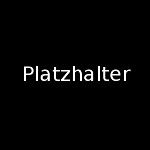
\includegraphics[scale=1.0]{spacer}
%		\caption{Optimaler Helligkeitsbereich/Bilder die verdeutlichen wann visodom failt und wann Projektion zu undeutlich wird}
%		\label{fig.optlight}
%	\end{center}
%	%\vspace*{-8mm}
%\end{figure}

%Anzumerken bleibt, dass eine Begrenzung der Leistung und damit auch der Helligkeit bei Laser-Projektoren durch die zulässige Laser-Klasse vorgegeben ist. Besonders im Bereich der tragbaren Projektoren sollte die Laser-Klasse 2\footnote{Klassifizierung nach EN 60825-1} nicht überschritten werden, da es sonst bei versehentlicher Betrachtung des Laserstrahls zu permanenten Schädigungen der Netzhaut kommen kann. Auch im Hinblick auf die \red[zuvor besprochene] Umgebungsausleuchtung sollte bei der Anwendung deshalb ein maximaler Abstand von etwa \red[TODO] zur Projektionsfläche nicht überschritten werden.\\

%Eine weitere Möglichkeit eine deutlichere Darstellung der visuellen Zusatzinformationen zu erreichen, wäre neben einer Kontrast- beziehungsweise Helligkeitserhöhung auch eine Erhöhung der Auflösung der Projektion. Der ShowWX ist auf eine Auflösung von 480p begrenzt, wodurch es besonders bei feineren Strukturen trotz der Laser-Technologie zu unscharfen Abbildungen kommen kann.\\

%\subsection{Raspberry Pi}
%Es zeigt sich, \red[TODO]\\
%Das gekapselte Projektionsmodul bestehend aus dem Raspberry Pi und dem Microvision ShowWX ist damit \red[nicht geeignet/vergleichbar mit/...]\\
%\red[Delay bzgl. raspberry -> Übertragung an anderen Rechner testen und Delay ebenfalls aufzeichnen\\]

%\section{Interaktion}
%Durch den minimalen aufgelösten Tiefenwert des Microsoft Kinect Sensors von \red[ABSTAND 0,5m?] ergibt sich eine Limitierung der aktuellen Systemkonfiguration bezüglich der Benutzerinteraktion. Um die Zeigerichtung robust erkennen zu können, ist es erforderlich, dass der Nutzer die Auswahl und Modifikation der Modellobjekte mit ausgestrecktem Arm durchführt. Eine kürzere minimale Distanz würde den Komfort bei der Eingabe deutlich erhöhen, da so die Interaktion bei verschiedenen Haltungen möglich wäre und der Benutzer bei längerer Interaktionsdauer entlastet werden würde.\\
%
%Der minimale Tiefenwert definiert darüber hinaus auch den minimalen Abstand zur Projektionsfläche, da sowohl der globalen als auch der lokalen Lokalisation bei Unterschreiten dieses Abstands keine Umgebungsinformationen mehr zur Verfügung stehen. Es ergibt sich daraus zusammen mit dem definierten maximalen Projektionsabstand der in \abb{fig.optdist} dargestellte optimale Anwendungsabstand.\\
%\red[Interaktionsbereich hier auch einzeichnen! Wand anstelle rotem Endbereich!?\\]
%\red[Empfehlung für Mindestabstand? Dann auch mit Kinect vergleichen und optimalen Betriebsbereich definieren; Bild, welches diesen darstellt?\\]

%\begin{figure}[!ht]
%	\begin{center}
%		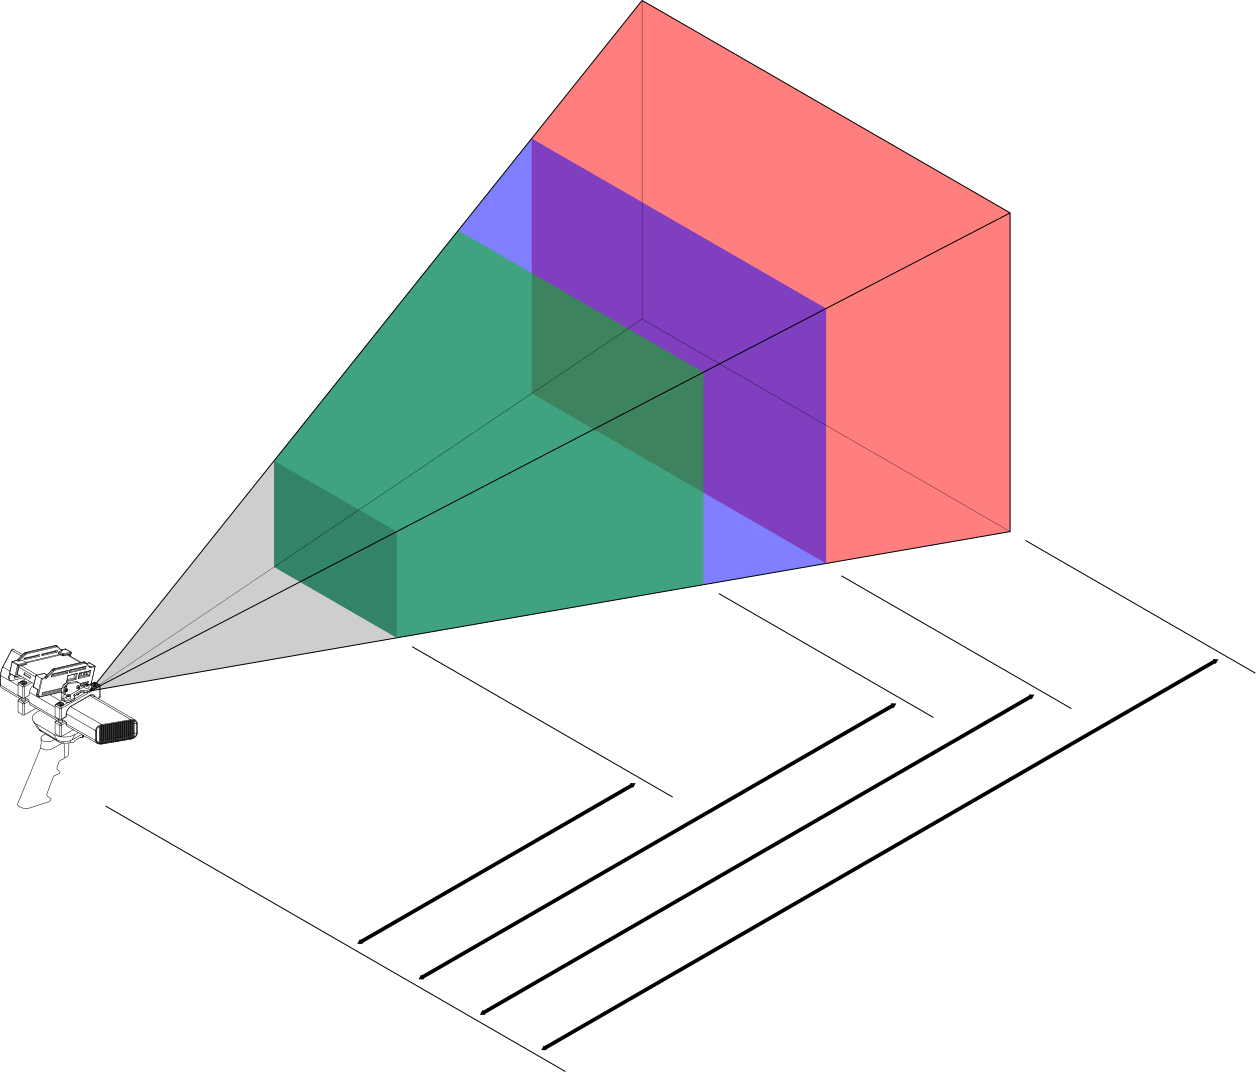
\includegraphics[scale=0.25]{anwendungsbereich}
%		\caption{Optimaler Abstand während der Verwendung des \kps{s}}
%		\label{fig.optdist}
%	\end{center}
%	%\vspace*{-8mm}
%\end{figure}


%\red[andere Struktur? Nicht Komponenten sondern Lokalisation, Projektion etc.?\\]
%
%\red[TODO:\\
%%Einleitender Absatz\\
%%Limitierungen der Hardware\\
%%Limitierungen der Lokalisation, global und lokal (Licht, features)\\
%%Limitierungen des Projektors (Lichtstärke, Auflösung etc.)\\
%Limitierungen in der Anwendung\\
%Limitierungen in der Rechenleistung\\
%]
%\section{Hardware}

%\section{Software}

%\section{Anwendung}










%\red[Allgemein]\\
%Gesamtsystem kalibriert;\\
%System ermöglicht Lokalisation und Darstellung visueller Zusatzinformationen;\\
%Anbindung an ROS ermöglicht Austausch verschiedener Module;\\
%
%\red[Datengrundlage beschreiben!?\\]
%
%\red[Lokalisationsverfahren beschreiben, globale und lokale unterscheiden, IMU+EKF nennen.]\\
%Selbstlokalisation durch Partikelfilter verwendet;\\
%Tracking basierend auf visueller Odometrie verwendet;\\
%Robustheit durch IMU und Kalman-Filter gesteigert;\\
%
%\red[Visualisierung der Modelldaten und Simulation der Projektorperspektive.]\\
%Projektion von Modelldaten, Projektor als inverse Kamera, die Modellszene betrachtet, eigentlich nicht mehr direkt invers dann;\\
%Grafische Benutzeroberfläche erstellt, welche die Funktionen zugänglich macht, ist aber für Anwendung nicht unbedingt erforderlich, dann muss vorher die Welt definiert werden;\\
%
%\red[Interaktion ermöglicht Modifikation der Datengrundlage durch Rückkopplung]\\
%Buttons integriert;\\
%%
%%\red[Bewertung]\\
%%Ergebnisse zusammenfassen\\
%Erweiterung -> Ground Truth über externes Lokalisationssystem bestimmen\\
%
%\red[Ausblick/Erweiterungen]\\
%Lokalisation und Visualisierung benötigen viel Rechenleistung!\\
%Anwendung unterliegt ein paar Einschränkungen, die jedoch im geplanten Anwendungsszenario keine Probleme machen sollten; Unter Berücksichtigung der Empfehlungen aus dem vorhergehenden Kapitel;\\
%
%Lokalisation\\
%Steigerung der Auflösung -> erhöhte Rechenleistung erforderlich\\
%-> Kinect V2;\\
%Kompass zur Lagebestimmung yaw -> deutliche Reduzierung der Partikelanzahl möglich;\\
%-> Könnte auch durch EKF die visuelle Odometrie unterstützen\\
%Ausreichend Features in der Umgebung erforderlich\\
%-> Modifizierter Ansatz, der weniger Features benötigt, da er zusätzlich RGB- und D-Bilder getrennt auswertet (statt zusammen wie fovis)\\
%Anpassung der Varianz im Sensormodell in Abhängigkeit der Entfernung\\
%
%Visualisierung\\
%Projektor mit geringer Helligkeit in ausgeleuchteten Räumen\\
%Höhere Helligkeit würde möglichen Projektionsabstand und Anwendungsbereich erweitern\\
%-> Aber, Laserklasse 2 als Begrenzung\\
%-> Aber visuelle Odometrie benötigt gute Ausleuchtung der Szene\\
%Raspberry Pi Performanz nochmal aufgreifen?\\
%-> Empfehlungen?\\
%Projektion auf beliebige Oberflächen/Untergründe\\
%-> Arbeiten siehe Stand der Technik\\
%-> Bimber - Embedded Entertainment with Smart Projectors\\
%-> Park - Kontrast erhöhung\\
%-> Wang - Relighting\\
%
%-> Bimber - Multi-Projector Techniques for Real Time... -> Architectural Projection\\
%
%Interaktion\\
%Minimal aufgelöster Tiefenwert von 0,5m\\
%-> Interaktion auf Dauer evtl. anstrengend\\
%-> Mindestabstand zur Wand -> Definiert mit maximalem Projektionsabstand (aus Projektor Specs) optimalen Anwendungsbereich (der Komponenten!?)\\
%-> Gestenerkennung -> Kinect V2 gut, da bessere Auflösung; Aber auch 0,5m\\
%-> InfrarotKamera für Nahbereich!? wie bei Molyneaux\\

%\red[aufgrund!]